\documentclass{article}
\usepackage{amsmath}
\usepackage{amssymb}
\usepackage{graphicx}
\usepackage{hyperref}
\usepackage[version=4]{mhchem}

\title{Problem 4}
\date{}

\begin{document}
\maketitle

\section*{Problem}
Triangle \(A B C\) is inscribed in the circle \(O\). Draw \(C D / / A B\). Draw tangent line through \(B\) to meet the extension of \(C D\) at \(P\). Show that \(P B \times C A=C B \times P D\).\\
\centering
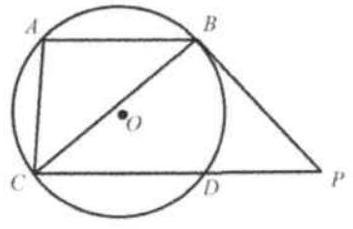
\includegraphics[width=\textwidth]{images/problem_image_1.jpg}

\section*{Solution}
Connect \(B D\). Since \(B P\) is tangent to circle \(O, \angle P B D=\angle B C D=\alpha\) (both angles face the same arc \(B D\) ).\\
Since \(A B / / C D, \angle B C D=\angle C B A=\alpha\).\\
So \(\angle P B D=\angle C B A=\alpha\).\\
Since points \(A, B, D\), and \(C\) are concyclic, \(\angle P D B=\angle C A B=\beta\).\\
Thus \(\triangle P D B \sim \triangle C A B\).\\
\centering
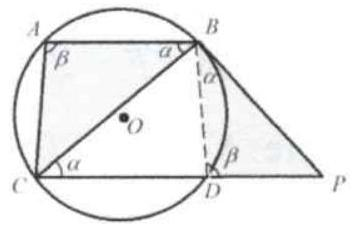
\includegraphics[width=\textwidth]{images/reasoning_image_1.jpg}

Thus \(\frac{A C}{P D}=\frac{C B}{P B} \quad \Rightarrow \quad P B \times C A=C B \times P D\).

\end{document}
